\chapter{Introduction}
%\chapter{Einleitung}

% \begin{itemize}
% 	\item general motivation for your work, context and goals.
% 	\item context: make sure to link where your work fits in
% 	\item problem: gap in knowledge, too expensive, too slow, a deficiency, superseded technology
% 	\item strategy: the way you will address the problem
% 	\item recommended length: 1-2 pages.
% \end{itemize}

Through stage lighting, lights or installations can be controlled to match a stage for a given event.
These installations include moving heads, spotlights, or even fog machines.
These individual stations are controlled several times per second with control signals from the light desk
to adapt them to the stage.

Wireless connections have advantages over wired solutions such as flexibility and cost-efficiency.
However, they also have their own limitations.
This thesis addresses approaches that could further optimise state-of-the-art solutions like Art-Net and DMX-512a.

\begin{figure}[h]
    \centering
    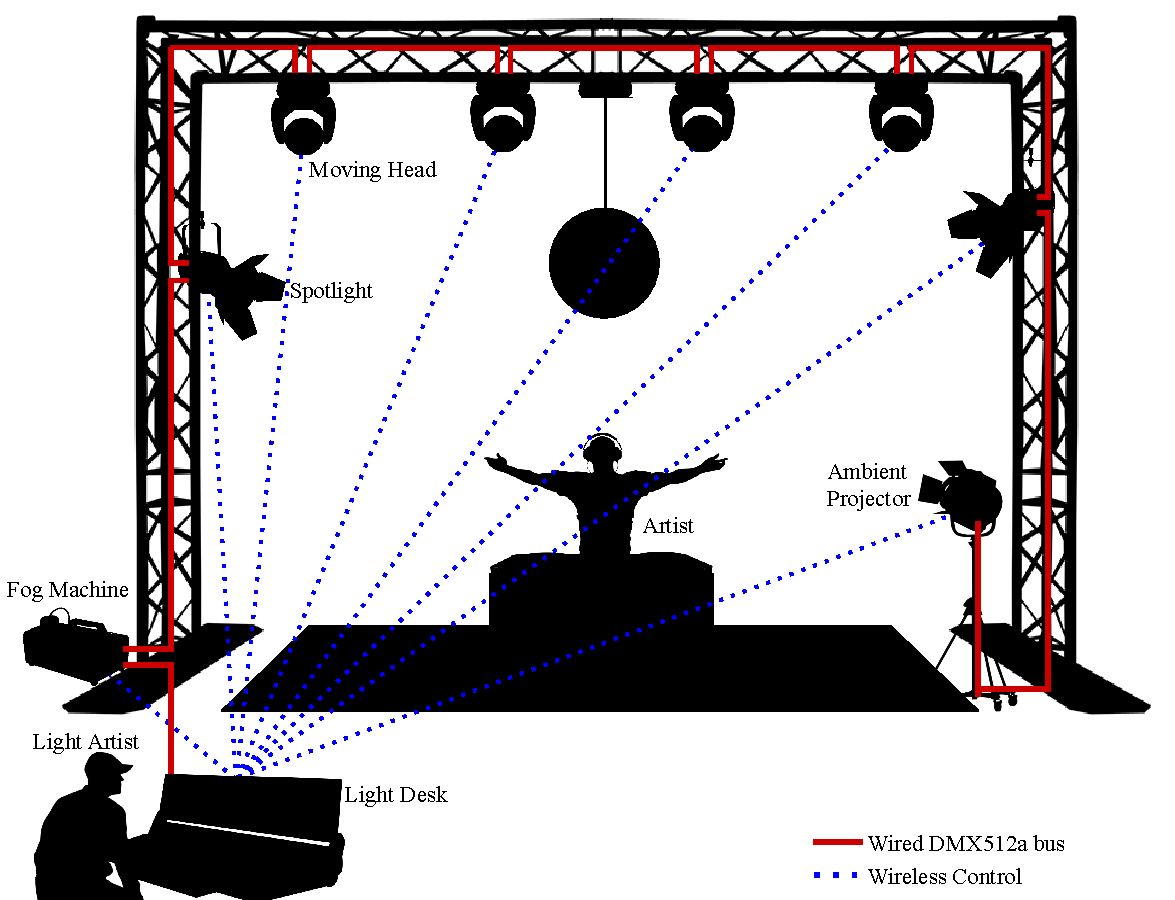
\includegraphics[scale=0.55]{figures/illustration.pdf}
    \label{fig:illustration}
    \caption{Illustration of a stage light installation}
\end{figure}

\section*{Motivation and Requirements}
% \begin{itemize}
% 	\item Reliability
% 	\item .. and why 100\% Reliability is not important (except pyrotechnics)
% 	\item Lower latency
% 	\item Synchronisation
% 	\item higher update frequency
% 	\item Range
% \end{itemize}

By sending very small packets with a high update frequency to many stations, 
the overhead associated with each transmission is significant.
In order to improve the properties of radio networks, a logic link layer approach,  
in contrast to the TCP/UDP and Wi-Fi stack, is chosen to reduce the overhead.
It will also be investigated whether the overhead 
can be reduced further by sending fewer broadcasts to all stations at the same time, compared to many individual unicasts.

The properties of the wired DMX-512a protocol solution are taken as a baseline.
The Update Frequency of 44 Hz of this old protocol is rather slow, compared to today's standards.
Nevertheless, they should not fall below 44 Hz, even with a high number of stations.
The reliability that is achieved with wired solutions is not feasible with radio technology,
but it should reach a success ratio of 99\%.
Due to the DMX data bus properties, the stations react synchronously, 
which is not the case with some wireless implementations using UDP unicasts. 
But this should be the case, because two lights that are positioned next to each other 
and do not react at the same time can disturb the imersion of the light show.

\section*{Challenges}

To counteract the lack of reliability, various protocols are presented and evaluated in the application layer.
These protocols exchange efficiency for reliability.
There will always be a possibility to build an even more reliable system with extremely complex hardware,
however, the focus of this thesis is to achieve results with low-cost hardware.
Lastly, the range should be at least 100 m and the hardware used should be as cost-effective as possible.

The utilized ESP-NOW protocol from the manufacturer Espressif is proprietary
and had to be investigated additionally due to the partly inaccurate or outdated documentation.

The complete control process takes place over microcontrollers, 
which have to be programmed in a fundamentally different way than ordinary programs.

\section*{Contribution}
% \begin{itemize}
% \item open source available on github [link]
% \item thought-provoking impulse for different approaches
% \item Protocol auf DL Layer/App Layer Ebene
% \item Art-Net baseline/DMX512a
% \item simulativ und experimentel untersucht
% \end{itemize}

This thesis introduces a number of protocols on the data link layer/application layer,
which offer promising improvements.
It turns out that broadcasts are preferable to unicasts.
The lack of reliability of broadcasts can at least be improved by adaptations in the application layer.
The results were validated in a small indoor test setup,
the test suite is publicly available on GitHub.\footnote{\url{https://github.com/senexger/bachelor}}
The analytical investigations suggest that the assumptions are also confirmed for larger setups.

\section*{Thesis Outline}

The thesis is divided into three main chapters.
Chapter 3 explains the 802.11 specifications family, the physical and the data link layer.
Existing light protocols are explained in order to better understand the new protocols that will be introduced later,
in addition, the EPS32 hardware and the associated ESP-NOW protocol are briefly shown.

Chapter 4 then specifies the various protocols developed and makes analytical assumptions and
additionally explains the given hardware.

Chapter 5 then introduces the methodology, how the measurement data was collected with a technical implementation.
Wireshark's measurements are analyzed and used to better understand the protocols.
Afterwards, the protocol data is further evaluated and compared with the analytical approaches.